% Combined pipeline: hashgrid lookup cells + feature column + SV head + MLP + sum.
% Layout:
%   Left:  two big cells (blue/green) with sample dots and bilinear lines
%   Mid:   feature column (lowered so feature+ellipsoid bbox center == cells' midpoint)
%   Right: MLP at the feature center (so feature→MLP arrow stays horizontal)
%   Above: d → [SC] → cyan ellipsoid
%   Far right: + merges cyan output and "residual" from MLP
\documentclass[tikz,border=4pt]{standalone}
\usepackage{tikz}
\usepackage{xcolor}
\usepackage{libertine}
\usepackage[libertine]{newtxmath}
\usepackage{amsmath}
\usetikzlibrary{positioning, calc, arrows.meta}

\begin{document}
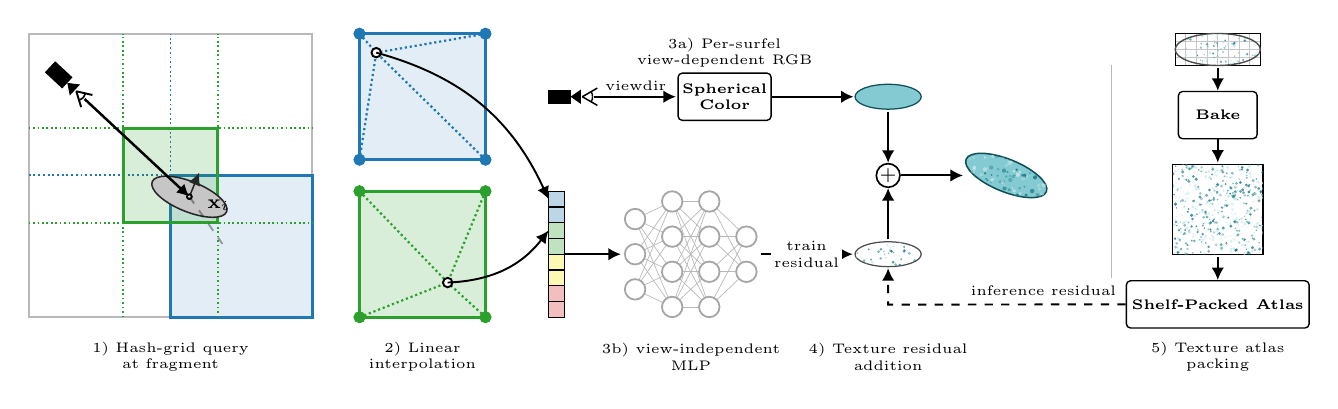
\begin{tikzpicture}[
  font=\sffamily\footnotesize,
  >={Latex[length=4.5pt,width=4.5pt]},
]

\definecolor{cBlue} {HTML}{1F77B4}
\definecolor{cGreen}{HTML}{2CA02C}
\definecolor{cLemon}{HTML}{F4ED00}
\definecolor{cRedB} {HTML}{D62728}
\definecolor{cCyan} {HTML}{1F9FAE}

% ============================================================================
% Scene-intersect diagram (on the LEFT). Scaled 0.6× to match the pipeline's
% vertical extent y∈[1.8, 5.4]; shifted so its right edge sits ~0.6 cm left of
% the pipeline cells (which start at x = 2.1).
% Local coords (0..6, 0..6) → absolute (-2.1..1.5, 1.8..5.4).
% ============================================================================
\begin{scope}[shift={(-2.1, 1.8)}, scale=0.6]
  % scene bbox
  \draw[gray!55, thick] (0,0) rectangle (6,6);

  % --- 2x2 coarse grid (BLUE) — bottom-right cell highlighted ---
  \draw[cBlue, densely dotted, line width=0.7pt] (3,0) -- (3,6);
  \draw[cBlue, densely dotted, line width=0.7pt] (0,3) -- (6,3);
  \fill[cBlue, opacity=0.13] (3,0) rectangle (6,3);
  \draw[cBlue, line width=1.1pt] (3,0) rectangle (6,3);

  % --- 3x3 finer grid (GREEN) — middle cell highlighted ---
  \foreach \x in {2,4} {\draw[cGreen, densely dotted, line width=0.6pt] (\x,0) -- (\x,6);}
  \foreach \y in {2,4} {\draw[cGreen, densely dotted, line width=0.6pt] (0,\y) -- (6,\y);}
  \fill[cGreen, opacity=0.18] (2,2) rectangle (4,4);
  \draw[cGreen, line width=1.1pt] (2,2) rectangle (4,4);

  % --- Surfel + intersection ---
  \coordinate (xint) at (3.4, 2.55);
  \begin{scope}[shift={(3.4,2.55)}, rotate=-22]
    \filldraw[gray!45, draw=gray!30!black, line width=0.55pt]
              (0,0) ellipse [x radius=0.85, y radius=0.32];
    \draw[->, gray!30!black, line width=0.55pt] (0,0) -- (0,0.55);
  \end{scope}

  % --- Camera glyph (new style): body + reverse-tip triangle + FOV with arc ---
  \pgfmathsetmacro{\apexx}{0.45}
  \pgfmathsetmacro{\apexy}{5.30}
  \pgfmathsetmacro{\dxx}{3.4}
  \pgfmathsetmacro{\dyy}{2.55}
  \pgfmathsetmacro{\vxL}{\dxx - \apexx}
  \pgfmathsetmacro{\vyL}{\dyy - \apexy}
  \pgfmathsetmacro{\vlen}{sqrt(\vxL*\vxL + \vyL*\vyL)}
  \pgfmathsetmacro{\uxL}{\vxL/\vlen}
  \pgfmathsetmacro{\uyL}{\vyL/\vlen}
  \pgfmathsetmacro{\camRot}{atan2(\uyL, \uxL)}

  % Glyph dimensions (local; the scene_intersect scope itself is scaled 0.6).
  \pgfmathsetmacro{\sicbw}{0.50}
  \pgfmathsetmacro{\sicbh}{0.32}
  \pgfmathsetmacro{\sictlen}{0.22}
  \pgfmathsetmacro{\sicgap}{0.04}
  \pgfmathsetmacro{\sicangDeg}{30}
  \pgfmathsetmacro{\sicarmLen}{0.35}
  \pgfmathsetmacro{\sicarcR}{0.20}
  \pgfmathsetmacro{\sicarmX}{\sicarmLen*cos(\sicangDeg)}
  \pgfmathsetmacro{\sicarmY}{\sicarmLen*sin(\sicangDeg)}
  \pgfmathsetmacro{\sicFovApexX}{\sicbw + \sictlen + \sicgap}
  \pgfmathsetmacro{\siccamOutX}{\sicFovApexX + \sicarcR + 0.04}

  % Ray-exit point in world coords (just past the FOV arc, along view dir).
  \pgfmathsetmacro{\rayWX}{\apexx + \siccamOutX*\uxL}
  \pgfmathsetmacro{\rayWY}{\apexy + \siccamOutX*\uyL}
  \coordinate (rayStart) at (\rayWX, \rayWY);

  % Ray from camera output toward xint
  \draw[black, line width=0.9pt, ->] (rayStart) -- (xint);

  % Camera glyph, rotated to align with the view direction
  \begin{scope}[shift={(\apexx, \apexy)}, rotate=\camRot]
    \fill[black] (0, -\sicbh/2) rectangle (\sicbw, \sicbh/2);
    \fill[black] (\sicbw, 0) -- (\sicbw + \sictlen,  \sicbh/2)
                             -- (\sicbw + \sictlen, -\sicbh/2) -- cycle;
    \pgfmathsetmacro{\fovx}{\sicFovApexX}
    \draw[black, line width=0.7pt] (\fovx, 0) -- (\fovx + \sicarmX,  \sicarmY);
    \draw[black, line width=0.7pt] (\fovx, 0) -- (\fovx + \sicarmX, -\sicarmY);
    \draw[black, line width=0.6pt]
      (\fovx + \sicarcR, 0) arc (0:\sicangDeg:\sicarcR);
    \draw[black, line width=0.6pt]
      (\fovx + \sicarcR, 0) arc (0:-\sicangDeg:\sicarcR);
  \end{scope}

  % intersection circle
  \draw[black, line width=0.7pt, fill=white] (xint) circle (0.05);
  \node[font=\sffamily\scriptsize, anchor=west]
    at ($(xint)+(0.18,-0.18)$) {$\mathbf{x}_i$};
  % faint continuation past the disk
  \draw[black, line width=0.7pt, dashed, opacity=0.35]
    (xint) -- ($(xint)+(0.7,-1.0)$);
\end{scope}

% ============================================================================
% Two big grid cells (left): blue (top) and green (bottom).
% ============================================================================
\pgfmathsetmacro{\szC}{1.6}   % cells halved (3.2 -> 1.6)

% Blue cell — top.  Cells shifted right so the gap to the feature column ≈ half a cell.
\begin{scope}[shift={(2.10,3.8)}]
  \fill[cBlue, opacity=0.13] (0,0) rectangle (\szC,\szC);
  \draw[cBlue, line width=1.1pt] (0,0) rectangle (\szC,\szC);
  \pgfmathsetmacro{\sx}{0.133*\szC}
  \pgfmathsetmacro{\sy}{0.850*\szC}
  \coordinate (sB) at (\sx,\sy);
  \draw[cBlue, densely dotted, line width=0.8pt] (0,0)      -- (sB);
  \draw[cBlue, densely dotted, line width=0.8pt] (\szC,0)    -- (sB);
  \draw[cBlue, densely dotted, line width=0.8pt] (0,\szC)    -- (sB);
  \draw[cBlue, densely dotted, line width=0.8pt] (\szC,\szC) -- (sB);
  \foreach \p in {(0,0),(\szC,0),(0,\szC),(\szC,\szC)} {
    \filldraw[cBlue] \p circle (0.07);
  }
  \draw[black, line width=0.7pt, fill=white] (sB) circle (0.06);
\end{scope}

% Green cell — bottom
\begin{scope}[shift={(2.10,1.8)}]
  \fill[cGreen, opacity=0.18] (0,0) rectangle (\szC,\szC);
  \draw[cGreen, line width=1.1pt] (0,0) rectangle (\szC,\szC);
  \pgfmathsetmacro{\sx}{0.700*\szC}
  \pgfmathsetmacro{\sy}{0.275*\szC}
  \coordinate (sG) at (\sx,\sy);
  \draw[cGreen, densely dotted, line width=0.8pt] (0,0)      -- (sG);
  \draw[cGreen, densely dotted, line width=0.8pt] (\szC,0)    -- (sG);
  \draw[cGreen, densely dotted, line width=0.8pt] (0,\szC)    -- (sG);
  \draw[cGreen, densely dotted, line width=0.8pt] (\szC,\szC) -- (sG);
  \foreach \p in {(0,0),(\szC,0),(0,\szC),(\szC,\szC)} {
    \filldraw[cGreen] \p circle (0.07);
  }
  \draw[black, line width=0.7pt, fill=white] (sG) circle (0.06);
\end{scope}

% ============================================================================
% Feature column.  Scaled down so its lower edge aligns with the green cell
% bottom (y=1.8). MLP scaled similarly; both centered at y=fCy=2.6.
% Cyan ellipsoid moves to y=4.6 to keep symmetry around + (y=3.6).
% ============================================================================
\pgfmathsetmacro{\fw}{0.20}                    % shrunk square side
\pgfmathsetmacro{\fxL}{4.50}
\pgfmathsetmacro{\fxR}{\fxL + \fw}
\pgfmathsetmacro{\fCy}{2.60}                   % feature center
\pgfmathsetmacro{\fyTop}{\fCy + 4*\fw}         % top edge of column

\foreach \i/\col in {0/cBlue, 1/cBlue,
                      2/cGreen, 3/cGreen,
                      4/cLemon, 5/cLemon,
                      6/cRedB,  7/cRedB}{
  \pgfmathsetmacro{\fyHi}{\fyTop - \i*\fw}
  \pgfmathsetmacro{\fyLo}{\fyHi - \fw}
  \fill[\col!30!white] (\fxL,\fyLo) rectangle (\fxR,\fyHi);
  \draw[black, line width=0.5pt] (\fxL,\fyLo) rectangle (\fxR,\fyHi);
}

% Curving arrows from cell sample dots to feature column entries.
\pgfmathsetmacro{\tBlueY}{\fyTop - 0.5*\fw}    % center of top blue square in feature
\pgfmathsetmacro{\tGreenY}{\fyTop - 2.5*\fw}   % center of top green square in feature
\coordinate (tBlue)  at (\fxL,\tBlueY);
\coordinate (tGreen) at (\fxL,\tGreenY);
\draw[->, black, line width=0.7pt]
  (sB) to[bend left=25, looseness=1.0]  (tBlue);
\draw[->, black, line width=0.7pt]
  (sG) to[bend right=25, looseness=1.0] (tGreen);

% ============================================================================
% MLP, centered at the feature column's y center (so the small arrow is flat)
% ============================================================================
% Plus position offset from MLP's right edge (shifted further right).
\pgfmathsetmacro{\plusXshift}{1.80}
% Vertical scale (keeps MLP lower-edge at y=1.8) and a separate, smaller
% horizontal scale to make the NN narrower → longer train-residual arrow.
\pgfmathsetmacro{\mlpK}{0.812}
\pgfmathsetmacro{\mlpKx}{0.65}
\pgfmathsetmacro{\mlpDX}{0.725*\mlpKx}
\pgfmathsetmacro{\mlpOx}{5.60}
\pgfmathsetmacro{\xA}{\mlpOx + 0*\mlpDX}
\pgfmathsetmacro{\xB}{\mlpOx + 1*\mlpDX}
\pgfmathsetmacro{\xC}{\mlpOx + 2*\mlpDX}
\pgfmathsetmacro{\xD}{\mlpOx + 3*\mlpDX}
\pgfmathsetmacro{\vs}{0.55*\mlpK}
\pgfmathsetmacro{\nr}{0.16*\mlpK}
\pgfmathsetmacro{\mlpY}{\fCy}
\pgfmathsetmacro{\mlpLeft}{\xA - \nr}
\pgfmathsetmacro{\mlpRight}{\xD + \nr}
\pgfmathsetmacro{\plusX}{\xD + \plusXshift}
\pgfmathsetmacro{\plusY}{3.60}

\foreach \i [count=\k from 0] in {-1, 0, 1}                { \coordinate (A\k) at (\xA, \mlpY + \i*\vs); }
\foreach \i [count=\k from 0] in {-1.5, -0.5, 0.5, 1.5}    { \coordinate (B\k) at (\xB, \mlpY + \i*\vs); }
\foreach \i [count=\k from 0] in {-1.5, -0.5, 0.5, 1.5}    { \coordinate (C\k) at (\xC, \mlpY + \i*\vs); }
\foreach \i [count=\k from 0] in {-0.5, 0.5}               { \coordinate (D\k) at (\xD, \mlpY + \i*\vs); }

\foreach \a in {0,1,2}    {\foreach \b in {0,1,2,3} {\draw[gray!55, line width=0.25pt] (A\a) -- (B\b);}}
\foreach \a in {0,1,2,3}  {\foreach \b in {0,1,2,3} {\draw[gray!55, line width=0.25pt] (B\a) -- (C\b);}}
\foreach \a in {0,1,2,3}  {\foreach \b in {0,1}     {\draw[gray!55, line width=0.25pt] (C\a) -- (D\b);}}

\foreach \name in {A0,A1,A2, B0,B1,B2,B3, C0,C1,C2,C3, D0,D1}{
  \fill[white] (\name) circle (\nr);
  \draw[gray!70, line width=0.65pt] (\name) circle (\nr);
}

% feature → MLP (small horizontal arrow at y=fCy)
\draw[black, line width=0.7pt, ->]
  (\fxR, \fCy) -- (\xA - \nr - 0.05, \fCy);

% ============================================================================
% SV head on top — d → [Spherical Color] → cyan ellipsoid
% Ellipsoid center y = fCy + 1.55 = 4.915  (so feature∪ellipsoid mid = 3.6)
% Entire SC + ellipsoid sits inside MLP horizontal width.
% ============================================================================
\pgfmathsetmacro{\svy}{4.60}     % cyan ellipsoid center (mirror of fCy across +)
\pgfmathsetmacro{\eXr}{0.42}     % matches grey surfel scale (0.85*0.6=0.51 abs)
\pgfmathsetmacro{\eYr}{\eXr / 2.66}

% Camera glyph: black body rectangle + reverse-tip triangle ("lens")
% + FOV angle with arc. Arrow exits the FOV cone toward SC.
\pgfmathsetmacro{\cbw}{0.28}        % body width
\pgfmathsetmacro{\cbh}{0.18}        % body height
\pgfmathsetmacro{\ctlen}{0.13}      % triangle (lens) length
\pgfmathsetmacro{\cgap}{0.02}       % gap from triangle base to FOV apex
\pgfmathsetmacro{\cangDeg}{30}      % half-FOV
\pgfmathsetmacro{\carmLen}{0.22}    % FOV arm length
\pgfmathsetmacro{\carcR}{0.13}      % FOV arc radius
\pgfmathsetmacro{\carmX}{\carmLen*cos(\cangDeg)}
\pgfmathsetmacro{\carmY}{\carmLen*sin(\cangDeg)}
\pgfmathsetmacro{\cbxL}{\fxL}
\pgfmathsetmacro{\cbxR}{\cbxL + \cbw}
\pgfmathsetmacro{\cbyB}{\svy - \cbh/2}
\pgfmathsetmacro{\cbyT}{\svy + \cbh/2}
\pgfmathsetmacro{\cFovApexX}{\cbxR + \ctlen + \cgap}
\pgfmathsetmacro{\camOutX}{\cFovApexX + \carcR + 0.02}
\coordinate (cFovApex) at (\cFovApexX, \svy);
\coordinate (cFovUp)   at ($(cFovApex) + (\carmX,  \carmY)$);
\coordinate (cFovDn)   at ($(cFovApex) + (\carmX, -\carmY)$);
\coordinate (camOut)   at (\camOutX, \svy);

% Cyan ellipsoid sits directly above the plus, so eCx = plusX.
\pgfmathsetmacro{\eCx}{\plusX}
\coordinate (svSurfel) at (\eCx, \svy);
\coordinate (ellW)     at (\eCx - \eXr, \svy);

% Spherical Color box centered between camera output and cyan ellipsoid west.
\node[draw=black, line width=0.5pt, rounded corners=1.5pt,
      fill=white, minimum width=10mm, minimum height=6mm,
      align=center, inner sep=1.5pt,
      font=\rmfamily\bfseries\fontsize{5}{6}\selectfont]
      (scBox) at ($(camOut)!0.5!(ellW)$) {Spherical\\Color};

% Arrow from camera output (just past the FOV cone) to SC.west
\draw[black, line width=0.6pt, ->]
  (camOut) -- ($(scBox.west) + (-0.02, 0)$);

% viewdir label riding the arrow
\node[anchor=south, font=\rmfamily\fontsize{5}{6}\selectfont, inner sep=2pt]
      at ($(camOut)!0.5!(scBox.west)$) {viewdir};

% Camera glyph (drawn after the arrow setup so it sits cleanly).
\fill[black] (\cbxL,\cbyB) rectangle (\cbxR,\cbyT);
\fill[black] (\cbxR,\svy) -- (\cbxR + \ctlen,\cbyT)
                          -- (\cbxR + \ctlen,\cbyB) -- cycle;
\draw[black, line width=0.55pt] (cFovApex) -- (cFovUp);
\draw[black, line width=0.55pt] (cFovApex) -- (cFovDn);
\draw[black, line width=0.5pt]
  ($(cFovApex) + (\carcR, 0)$) arc (0:\cangDeg:\carcR);
\draw[black, line width=0.5pt]
  ($(cFovApex) + (\carcR, 0)$) arc (0:-\cangDeg:\carcR);

% SC → cyan
\draw[black, line width=0.6pt, ->]
  (scBox.east) -- ($(svSurfel) + (-\eXr - 0.02, 0)$);

\begin{scope}[shift={(svSurfel)}]
  \filldraw[fill=cCyan!55!white, draw=cCyan!50!black, line width=0.45pt]
    (0,0) ellipse [x radius=\eXr, y radius=\eYr];
\end{scope}

% ============================================================================
% "+" merge of cyan output and MLP residual
% ============================================================================
% \plusX / \plusY already defined earlier in the file (above the MLP block).
\node[draw=black, line width=0.6pt, circle, inner sep=0pt,
      minimum size=3mm, fill=white,
      font=\sffamily\scriptsize] (plus) at (\plusX, \plusY) {$+$};

% cyan (above) → + (straight down)
\draw[black, line width=0.7pt, ->]
  ($(svSurfel) + (0, -\eYr - 0.03)$) -- (plus.north);

% Textured residual ellipse — directly below the plus, same size as cyan.
\coordinate (textSurf) at (\plusX, \mlpY);
\begin{scope}[shift={(textSurf)}]
  \draw[black!70, line width=0.45pt] (0,0) ellipse [x radius=\eXr, y radius=\eYr];
  \begin{scope}
    \clip (0,0) ellipse [x radius=\eXr, y radius=\eYr];
    \pgfmathsetseed{7}
    \foreach \i in {1,...,45} {
      \pgfmathsetmacro{\rx}{(rand)*\eXr}
      \pgfmathsetmacro{\ry}{(rand)*\eYr}
      \pgfmathsetmacro{\rs}{0.008 + rnd*0.013}
      \pgfmathsetmacro{\rop}{0.30 + rnd*0.55}
      \pgfmathsetmacro{\rshade}{rnd}
      \ifdim \rshade pt < 0.5pt
        \fill[cCyan!75!black, opacity=\rop] (\rx,\ry) circle (\rs);
      \else
        \fill[cCyan!25!white, opacity=\rop] (\rx,\ry) circle (\rs);
      \fi
    }
  \end{scope}
\end{scope}

% textured residual → +  (straight up)
\draw[black, line width=0.7pt, ->]
  ($(textSurf) + (0, \eYr + 0.03)$) -- (plus.south);

% MLP → "train\nresidual" → textured residual (horizontal)
\draw[black, line width=0.7pt, ->]
  (\xD + \nr + 0.05, \mlpY) -- ($(textSurf) + (-\eXr - 0.03, 0)$)
  node[pos=0.5, font=\rmfamily\fontsize{5}{6}\selectfont,
       align=center, fill=white, inner sep=1pt]
  {train\\residual};

% ============================================================================
% Output splat: cyan surfel + superimposed noise, drawn at the same -22° angle
% as the surfel in the scene-intersect diagram.
% ============================================================================
\pgfmathsetmacro{\oXr}{0.55}
\pgfmathsetmacro{\oYr}{\oXr / 2.66}
\coordinate (outSurfel) at (\plusX + 1.50, \plusY);

\draw[black, line width=0.7pt, ->]
  (plus.east) -- ($(outSurfel) + (-0.55, 0)$);

\begin{scope}[shift={(outSurfel)}, rotate=-22]
  % cyan body
  \filldraw[fill=cCyan!55!white, draw=cCyan!50!black, line width=0.55pt]
    (0,0) ellipse [x radius=\oXr, y radius=\oYr];
  % superimposed noise, clipped to the ellipse
  \begin{scope}
    \clip (0,0) ellipse [x radius=\oXr, y radius=\oYr];
    \pgfmathsetseed{42}
    \foreach \i in {1,...,90} {
      \pgfmathsetmacro{\rx}{(rand)*\oXr}
      \pgfmathsetmacro{\ry}{(rand)*\oYr}
      \pgfmathsetmacro{\rs}{0.012 + rnd*0.018}
      \pgfmathsetmacro{\rop}{0.30 + rnd*0.55}
      \pgfmathsetmacro{\rshade}{rnd}
      \ifdim \rshade pt < 0.5pt
        \fill[cCyan!75!black, opacity=\rop] (\rx,\ry) circle (\rs);
      \else
        \fill[cCyan!25!white, opacity=\rop] (\rx,\ry) circle (\rs);
      \fi
    }
  \end{scope}
\end{scope}

% ============================================================================
% Bake pipeline (right side), scaled so its vertical extent matches the
% main pipeline (y ∈ [1.80, 5.40]).
%   With equal-length (0.70) arrows: local y ∈ [-2.84, 2.82] (height 5.66).
%   scale = 3.60/5.66 ≈ 0.636; shift = (12.0, 3.61).
% ============================================================================
\begin{scope}[shift={(13.0, 3.61)}, scale=0.636]
  % --- TOP: bbox + grid + textured horizontal ellipsoid ---
  \pgfmathsetmacro{\bboxW}{1.70}
  \pgfmathsetmacro{\bboxH}{0.64}
  \pgfmathsetmacro{\bboxCx}{0.0}
  \pgfmathsetmacro{\bboxCy}{2.50}
  \pgfmathsetmacro{\bxL}{\bboxCx - \bboxW/2}
  \pgfmathsetmacro{\bxR}{\bboxCx + \bboxW/2}
  \pgfmathsetmacro{\byB}{\bboxCy - \bboxH/2}
  \pgfmathsetmacro{\byT}{\bboxCy + \bboxH/2}
  \pgfmathsetmacro{\gridDX}{\bboxW/8}
  \pgfmathsetmacro{\gridDY}{\bboxH/4}
  \foreach \i in {1,...,7} {
    \pgfmathsetmacro{\xpos}{\bxL + \i*\gridDX}
    \draw[gray!45, line width=0.3pt] (\xpos, \byB) -- (\xpos, \byT);
  }
  \foreach \i in {1,...,3} {
    \pgfmathsetmacro{\ypos}{\byB + \i*\gridDY}
    \draw[gray!45, line width=0.3pt] (\bxL, \ypos) -- (\bxR, \ypos);
  }
  \draw[black, line width=0.5pt] (\bxL, \byB) rectangle (\bxR, \byT);

  \pgfmathsetmacro{\eXrT}{0.85}
  \pgfmathsetmacro{\eYrT}{\eXrT/2.66}
  \coordinate (eCB) at (\bboxCx, \bboxCy);
  \begin{scope}[shift={(eCB)}]
    \draw[black!70, line width=0.5pt] (0,0) ellipse [x radius=\eXrT, y radius=\eYrT];
    \begin{scope}
      \clip (0,0) ellipse [x radius=\eXrT, y radius=\eYrT];
      \pgfmathsetseed{42}
      \foreach \i in {1,...,110} {
        \pgfmathsetmacro{\rx}{(rand)*\eXrT}
        \pgfmathsetmacro{\ry}{(rand)*\eYrT}
        \pgfmathsetmacro{\rs}{0.011 + rnd*0.017}
        \pgfmathsetmacro{\rop}{0.30 + rnd*0.55}
        \pgfmathsetmacro{\rshade}{rnd}
        \ifdim \rshade pt < 0.5pt
          \fill[cCyan!75!black, opacity=\rop] (\rx,\ry) circle (\rs);
        \else
          \fill[cCyan!25!white, opacity=\rop] (\rx,\ry) circle (\rs);
        \fi
      }
    \end{scope}
  \end{scope}

  % --- bake box ---
  \pgfmathsetmacro{\bakeY}{1.19}     % all three vertical arrows = 0.70
  \node[draw=black, line width=0.5pt, rounded corners=1.5pt,
        fill=white, minimum width=10mm, minimum height=6mm,
        align=center, inner sep=2pt,
        font=\rmfamily\bfseries\fontsize{5}{6}\selectfont]
        (bake) at (\bboxCx,\bakeY) {Bake};
  \draw[black, line width=0.7pt, ->]
    (\bboxCx,\byB - 0.04) -- (bake.north);

  % --- large noise square ---
  \pgfmathsetmacro{\sqSz}{1.80}
  \pgfmathsetmacro{\sqCy}{-0.70}
  \pgfmathsetmacro{\sqL}{\bboxCx - \sqSz/2}
  \pgfmathsetmacro{\sqR}{\bboxCx + \sqSz/2}
  \pgfmathsetmacro{\sqB}{\sqCy - \sqSz/2}
  \pgfmathsetmacro{\sqT}{\sqCy + \sqSz/2}
  \draw[black, line width=0.7pt, ->]
    (bake.south) -- (\bboxCx, \sqT + 0.04);
  \draw[black, line width=0.5pt] (\sqL,\sqB) rectangle (\sqR,\sqT);
  \begin{scope}
    \clip (\sqL,\sqB) rectangle (\sqR,\sqT);
    \pgfmathsetseed{42}
    \foreach \i in {1,...,500} {
      \pgfmathsetmacro{\rx}{\bboxCx + (rand)*\sqSz/2}
      \pgfmathsetmacro{\ry}{\sqCy + (rand)*\sqSz/2}
      \pgfmathsetmacro{\rs}{0.013 + rnd*0.022}
      \pgfmathsetmacro{\rop}{0.30 + rnd*0.55}
      \pgfmathsetmacro{\rshade}{rnd}
      \ifdim \rshade pt < 0.5pt
        \fill[cCyan!75!black, opacity=\rop] (\rx,\ry) circle (\rs);
      \else
        \fill[cCyan!25!white, opacity=\rop] (\rx,\ry) circle (\rs);
      \fi
    }
  \end{scope}

  % --- shelf-packed atlas box ---
  \pgfmathsetmacro{\spaY}{-2.59}
  \node[draw=black, line width=0.5pt, rounded corners=1.5pt,
        fill=white, minimum width=14mm, minimum height=6mm,
        align=center, inner sep=2pt,
        font=\rmfamily\bfseries\fontsize{5}{6}\selectfont]
        (spa) at (\bboxCx,\spaY)
        {Shelf-Packed Atlas};
  \draw[black, line width=0.7pt, ->]
    (\bboxCx,\sqB - 0.04) -- (spa.north);
\end{scope}

% ============================================================================
% Grey vertical separator between main pipeline (left) and bake (right).
% ============================================================================
\draw[gray!55, line width=0.6pt]
  (11.65, 2.30) -- (11.65, 5.00);

% ============================================================================
% Dashed inference path: shelf-packed atlas → left → up into the textured
% residual ellipse from below.
% ============================================================================
\draw[black, dashed, line width=0.7pt, ->]
  (spa.west) -- (\plusX, 1.96) -- ($(textSurf) + (0, -\eYr - 0.02)$);

% Inference residual label — joined to where the dashed arrow leaves the atlas.
\node[anchor=east, font=\rmfamily\fontsize{5}{6}\selectfont,
      inner sep=1pt]
      at ($(spa.west) + (-0.08, 0.17)$) {inference residual};

% ============================================================================
% Annotations / step labels
% ============================================================================
\node[font=\rmfamily\fontsize{5}{6}\selectfont, align=center]
  at (-0.30, 1.30){1) Hash-grid query\\at fragment};

\node[font=\rmfamily\fontsize{5}{6}\selectfont, align=center]
  at (2.90, 1.30) {2) Linear\\interpolation};

\node[font=\rmfamily\fontsize{5}{6}\selectfont, align=center]
  at (6.31, 1.30) {3b) view-independent\\MLP};

\node[font=\rmfamily\fontsize{5}{6}\selectfont, align=center]
  at (\plusX, 1.30) {4) Texture residual\\addition};

\node[font=\rmfamily\fontsize{5}{6}\selectfont, align=center]
  at (13.0, 1.30) {5) Texture atlas\\packing};

\node[font=\rmfamily\fontsize{5}{6}\selectfont, align=center]
  at (scBox.north) [yshift=2.5mm] {3a) Per-surfel\\view-dependent RGB};

\end{tikzpicture}
\end{document}
